\documentclass[aspectratio=169]{beamer}
%\documentclass[notes]{beamer}       % print frame + notes
%\documentclass[notes=only]{beamer}   % only notes
%\documentclass{beamer}              % only frames

% for themes, etc.
\mode<presentation>
\usetheme{Madrid} 
\usecolortheme{crane}

%\usepackage{times}  % fonts are up to you
% The usual suspects
\usepackage{multirow, booktabs, dcolumn, color, graphicx} % Tables\usepackage{graphicx}
% Strikethrough text
\usepackage{soul}
% Adjust box to fit tabulars
\usepackage{adjustbox}
% Embed video
\usepackage{media9}
% For notes
\usepackage{pgfpages}
%\setbeameroption{hide notes} % Only slides
%\setbeameroption{show only notes} % Only notes
\setbeameroption{hide notes} % Both
% Video
\usepackage{multimedia}


% The table highlighting for hypothesis discussion.
\usepackage[beamer,customcolors]{hf-tikz}
\usetikzlibrary{calc}


% To use background images
\newenvironment{colorframe}[2][]{%
\setbeamercolor{background canvas}{bg=#1}
\begin{frame}\color{white}}
{\end{frame}}

% To set the hypothesis highlighting boxes red.
\tikzset{hl/.style={
    set fill color=red!80!black!40,
    set border color=red!80!black,
  },
}

% Set Graphics folder
\graphicspath{{./figures/}}


% these will be used later in the title page
\title{Networks}
\subtitle{In Class Exercise} % Sweet child of mine
\author{Irfan Kanat}
\institute[CBS]{{Department of Digitization}\\ Copenhagen Business School}
\date{\today}



\begin{document}

% this prints title, author etc. info from above
\begin{frame}

	\titlepage

\end{frame}


\begin{frame}
	\frametitle{Group Activity: Exercise}
    
    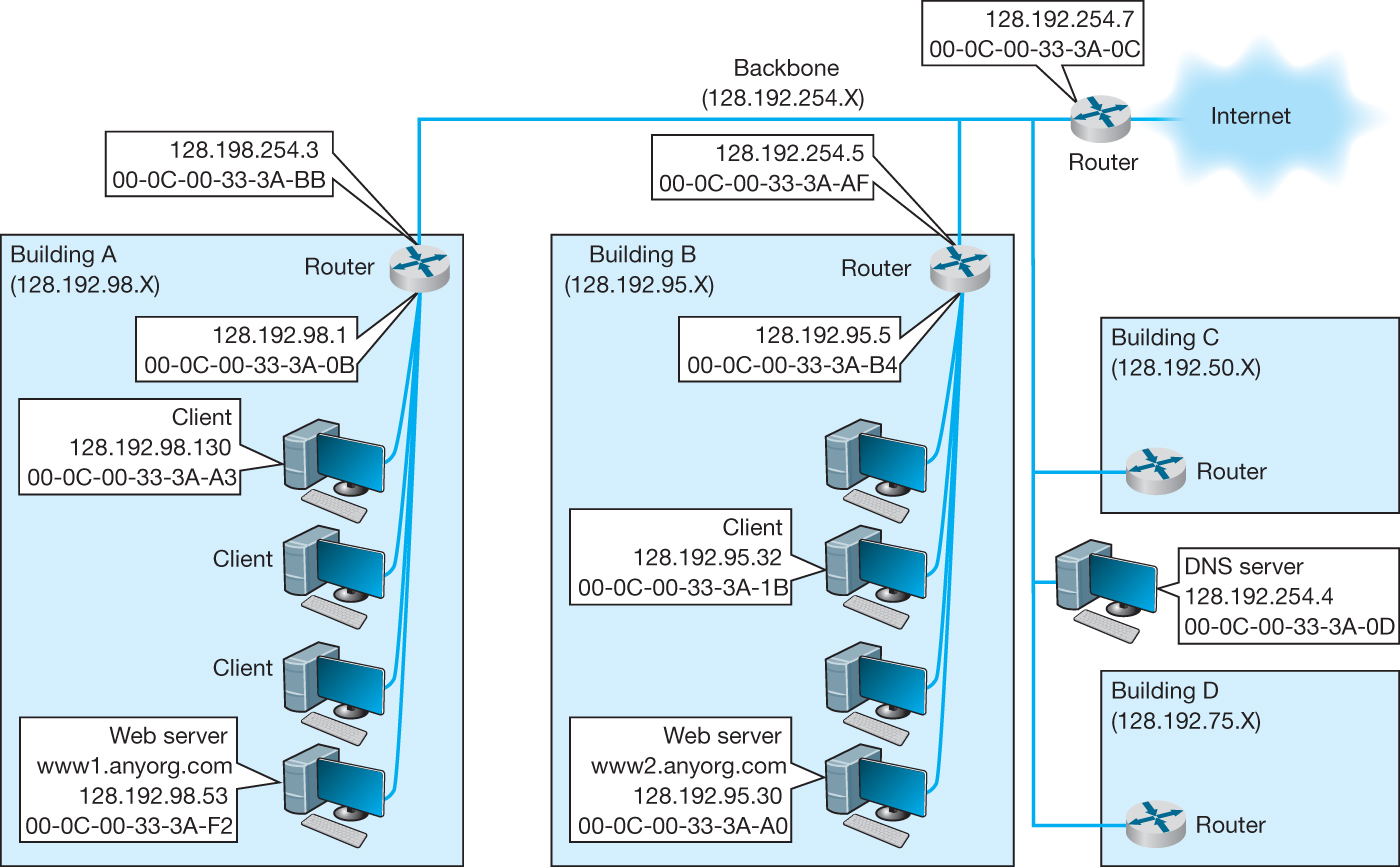
\includegraphics[width = \textwidth, height = .85\textheight, keepaspectratio]{figures/RoutingExercise.jpg}

\end{frame}


\begin{frame}[t]
	\frametitle{Exercise Case 1}
    
    CASE: Client (128.192.98.130) requests a web page from server (www1.anyorg.com) \vspace{1em}

    \only<2,4>{Client knows the server's IP and Ethernet Addresses \vspace{1em}

    List out the steps in getting the request to the server starting from client. \vspace{1em}}

    \only<3>{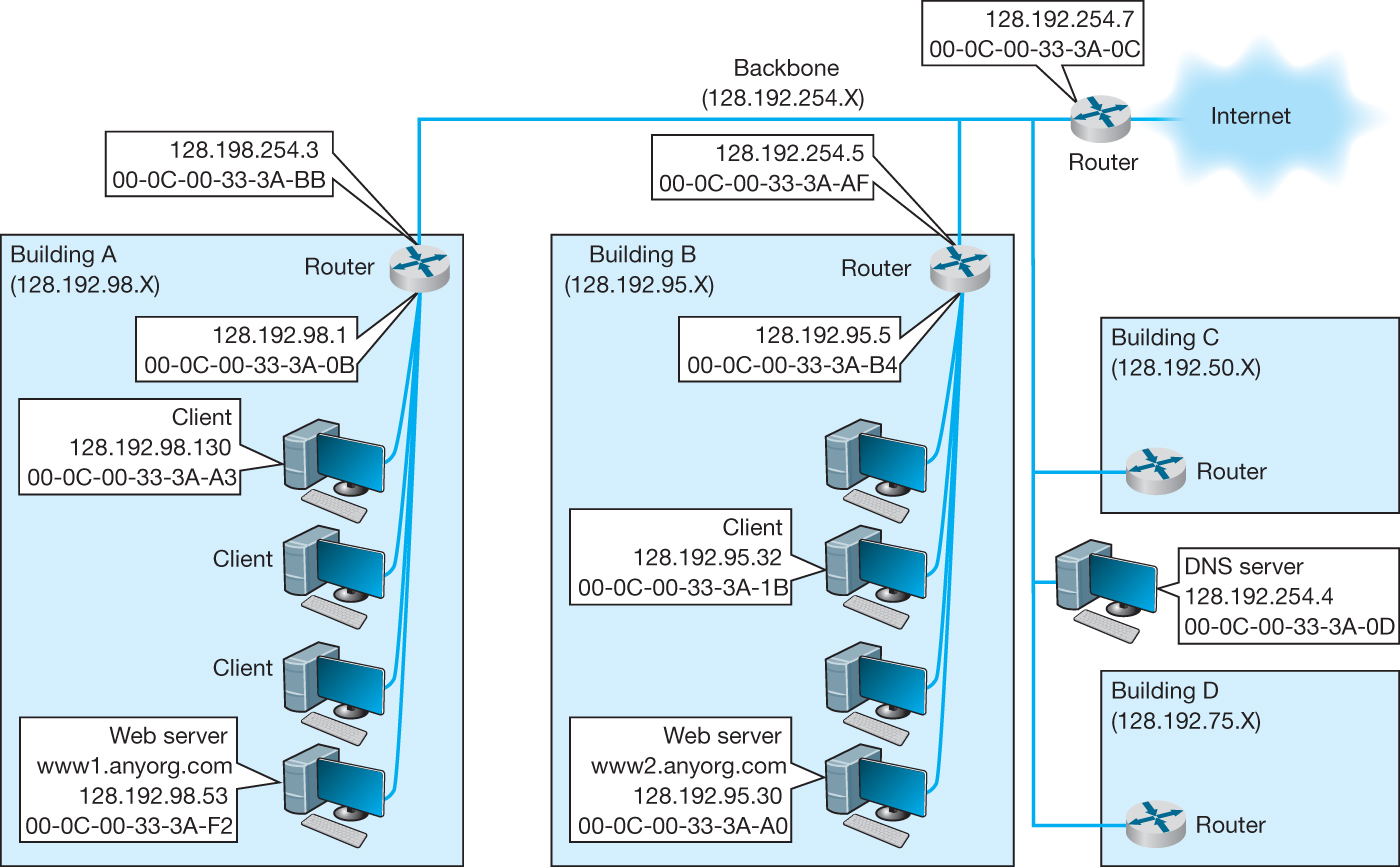
\includegraphics[width = .7\textwidth]{figures/RoutingExercise.jpg} }

    \only<4>{
    \begin{enumerate}
    	\item Create a package with all layers (HTTP, TCP, IP, MAC)
    	\item Destination IP address is set as 128.192.98.53
    	\item Client realizes it is on the same network
    	\item Adds the server's MAC address as the destination address (00-0C-00-33-3A-F2)
    	\item Switch (router) sees the MAC address and forwards it to server
    	\item Server receives the package 
    \end{enumerate}
    }

\end{frame}

\note{This one is for demonstration purposes. It is ok if the students miss a few steps here and there. Understanding the level of detail requested is not easy. We want them to learn so they can solve the subsequent cases.}


\begin{frame}[t]
	\frametitle{Exercise Case 2}
    
    CASE: Server (www1.anyorg.com) responds to client (128.192.98.130) \vspace{1em}

    \only<2,4>{List out the steps in getting the response to the client starting from server. \vspace{1em}}

    \only<3>{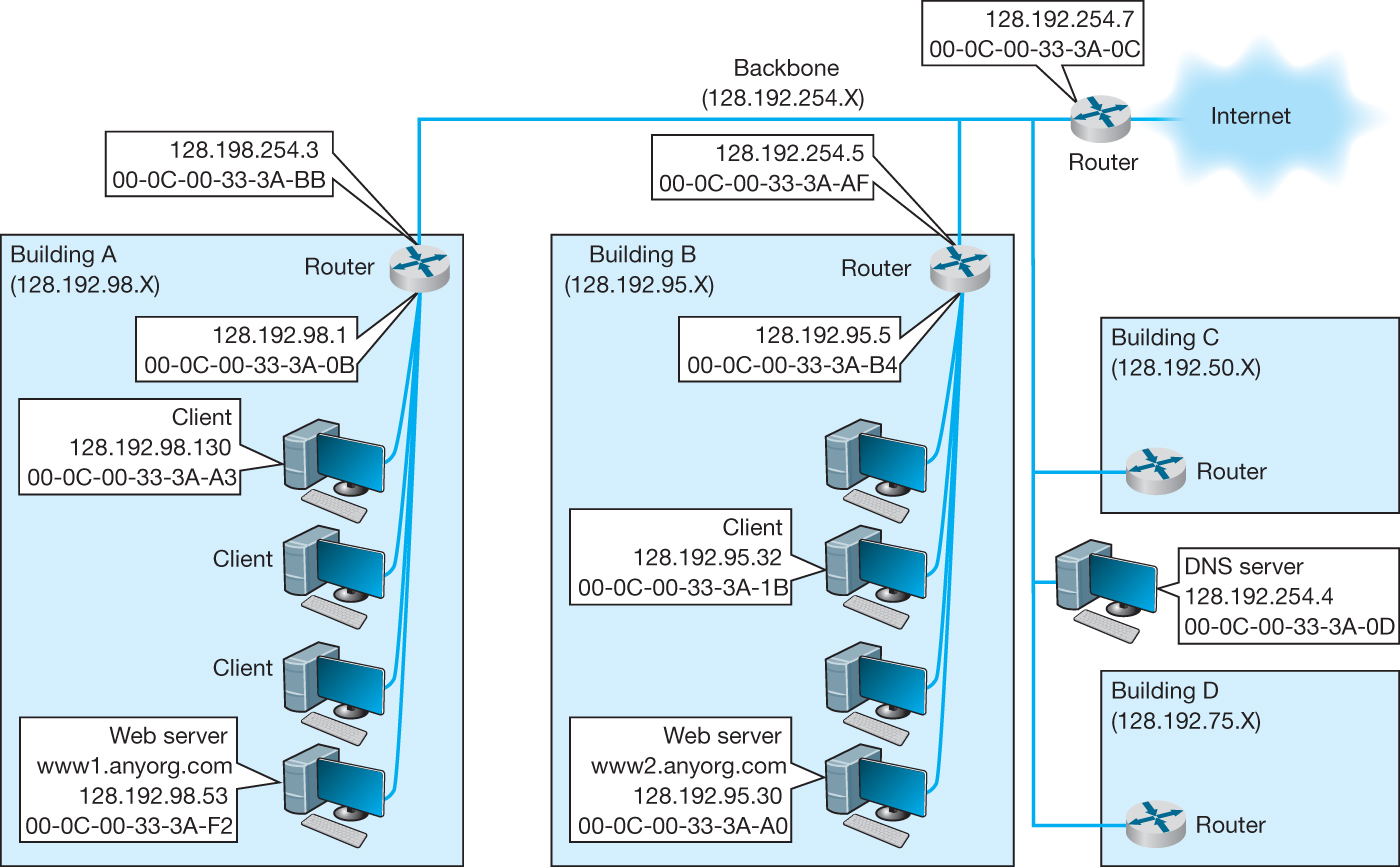
\includegraphics[width = .7\textwidth]{figures/RoutingExercise.jpg} }

    \only<4>{
    \begin{enumerate}
    	\item package received, goes up through the stack (MAC, IP, TCP, HTTP)
    	\item Prepare HTTP response with proper HTML web page (HTTP, TCP, IP, MAC)
    	\item Destination IP address is set as 128.192.98.130
    	\item Server realizes it is the same network.
    	\item Adds the client's MAC address as the destination (00-0C-00-33-3A-A3)
    	\item Switch (router) sees the MAC address and forwards it to client
    	\item Client receives the package 
    \end{enumerate}
    }

\end{frame}

\note{Essentially the same as before}


\begin{frame}[t]
	\frametitle{Exercise Case 3}
    
    CASE: Client (128.192.98.130) requests a web page from www2.anyorg.com.

    \only<2>{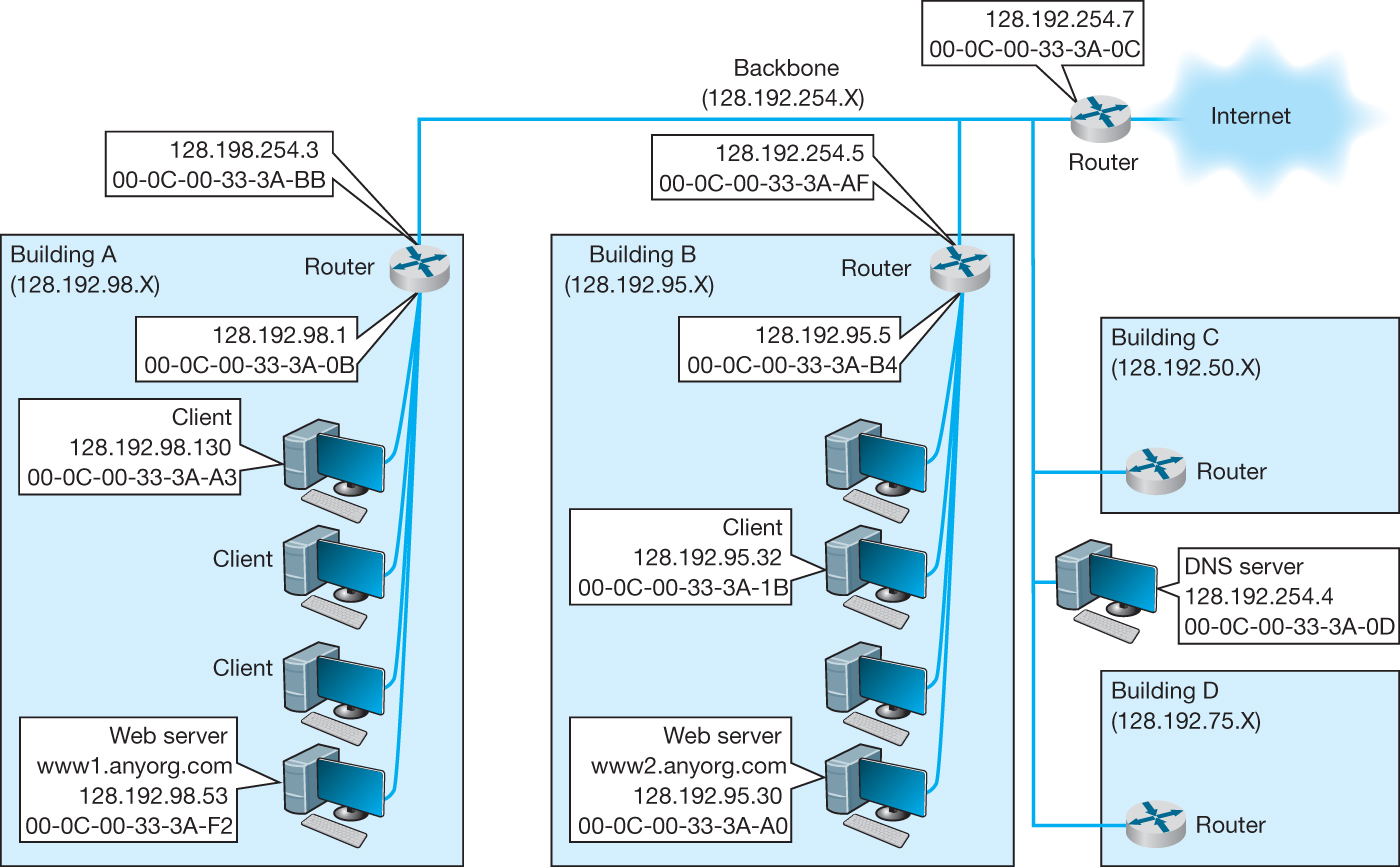
\includegraphics[width = .7\textwidth]{figures/RoutingExercise.jpg} }

    \only<3>{
    \begin{enumerate}
    	\item Create a package with all layers (HTTP, TCP, IP, MAC)
    	\item Destination IP address is set as 128.192.95.30
    	\item Client realizes it is not on the same network
    	\item Destination MAC address is set for the Gateway router (00-0C-00-33-3A-0B)
    	\item Router receives the package (it is the L2 destination)
    	\item Router removes L2 header
    	\item Router determines next node (Router Table)
    	\item Creates a new L2 header with next router MAC address (00-0C-00-33-3A-B4)
    	\item Second router receives 
    	\item Determines destination for local delivery (IP)
    	\item Replaces L2 header (MAC set to server's 00-0C-00-33-3A-A0)
    	\item Server receives the package.
    \end{enumerate}
    }    

\end{frame}


\begin{frame}
	\frametitle{Case 3: A picture is worth a thousand words}
    
    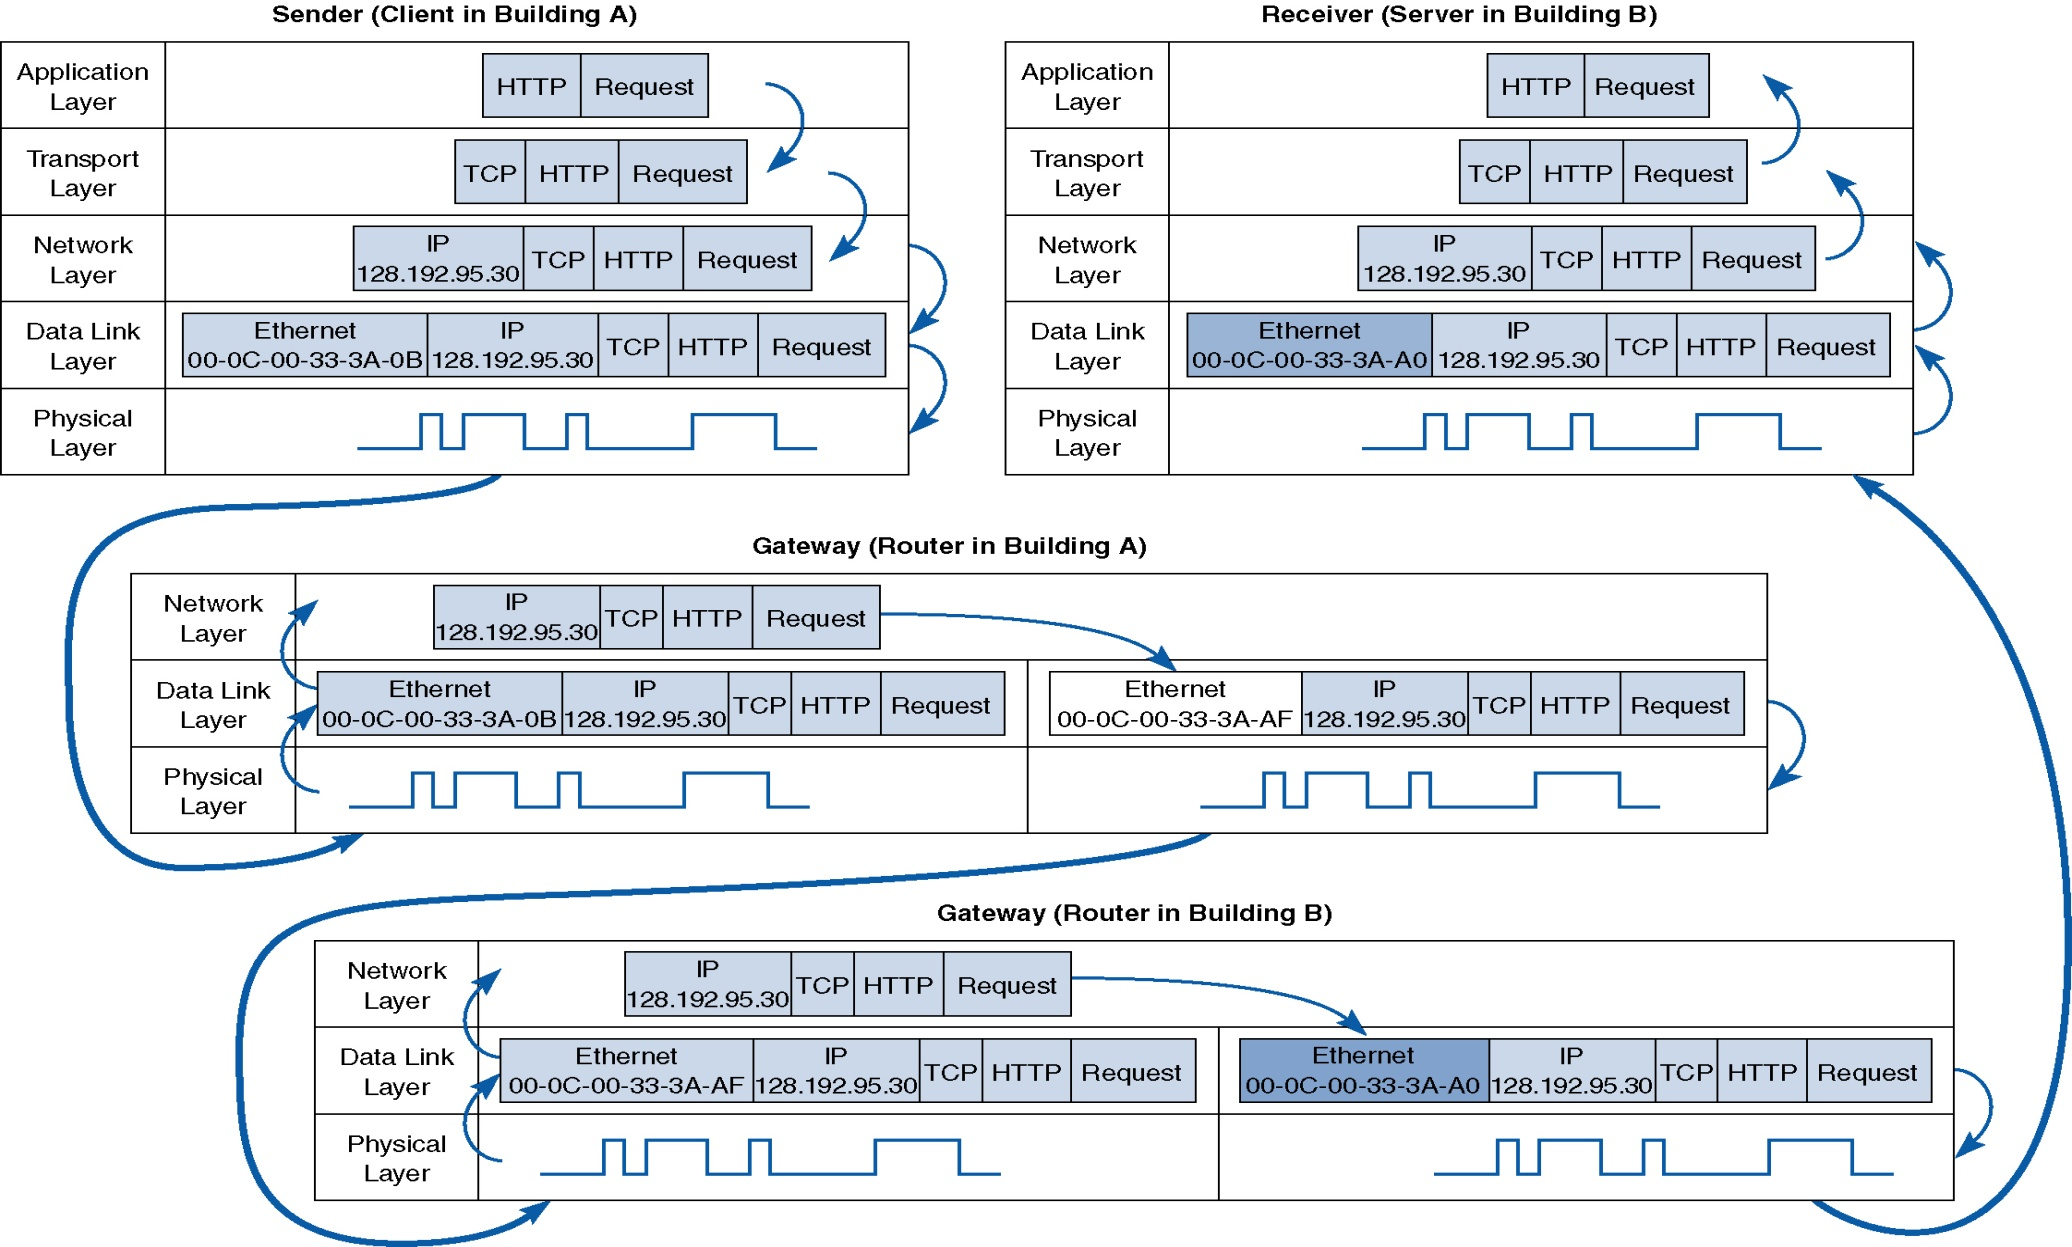
\includegraphics[width = \textwidth, height = .7\textheight, keepaspectratio]{figures/PackageThroughLayers.jpg}

\end{frame}


\end{document}
